\subsection{Jet deflection}

Angular deflection of the jet relative to its initial direction due to momentum transfer with the medium can be used as a direct probe of the QGP. 
Jet deflection can be measured by coincidence observables, in which an axis is determined by a hard reference object, and the deflection of the jet recoiling from hard object is measured relative to that axis. Such scattering measurements, carried out over a wide range in energy and resolution scale, can be used to explore the microscopic structure of the QGP. Modification of the rate of rare, large-angle jets with respect to the hard reference object in nuclear collisions compared to the production rate in vacuum may arise from the scattering off quasi-particles (quarks and gluons or composite objects) of the QGP, thereby probing their nature~\cite{DEramo:2012uzl}. In addition, the recoil jet distribution at small recoil angles relative to the reference axis (the axis of the hard object selected at the opposite hemisphere) may be modified by soft multiple scattering in the QGP, which can be used to extract the jet transport parameter $\hat{q}$ by comparison to models~\cite{Chen:2016vem}.

Measurements of the angular distribution of jets relative to a reference axis have been reported for either dijet, photon-jet, Z$^{0}$-jet and hadron-jet coincidences, at RHIC~\cite{Adamczyk:2017yhe} and LHC ~\cite{Adam:2015doa,Sirunyan:2017jic,Sirunyan:2017qhf,Chatrchyan:2012nia,Aaboud:2017eww}. 
These current measurements exhibit no significant evidence of in-medium modification of angular distributions, both at small and large angles to the reference axis. While they impose constraints on the magnitude of in-medium scattering effects, their statistical precision is limited. Measurements during HL-LHC will either discover in-medium modification to the recoil jet angular distributions, or improve these constraints substantially.

%Jets are complex dynamical objects.
%The shower of an energetic jet develops over an extended time interval, with the decoherence time of radiation in the shower correlated with its momentum scale and angle~\cite{Andrews:2018jcm}. Jet quenching arises from modification of this radiation pattern, due to scatterings with quarks and gluons in the medium and the quantum-mechanical interference between medium-induced and vacuum processes.
%In-medium angular deflection corresponds to coherent scattering of a highly virtual parton prior to development of the jet shower. However, deflection of a decoherent branch of the shower can also occur~\cite{DEramo:2018eoy}, resulting in both broadening of the jet shower and overall deflection of the jet direction. 

There is an intensive ongoing effort to develop analysis tools and calculable approaches that discriminate the various contributions to in-medium jet deflection and shower modification, in both experiment and theory~\cite{Andrews:2018jcm} (see Sec.~\ref{sec:preceloss} and~\ref{sec:jetsub}). In this section we focus solely on jet-centroid deflection measurements, without consideration of the effects of shower broadening or other shower modification (see Sec.~\ref{sec:jetsub}). Measurements of both classes of jet quenching observable must ultimately be interpretable in a single consistent picture, but such an approach is beyond current experimental and theoretical capabilities. %[{\it \color{blue} MV: shall we move this to introduction of the chapter?\color{black}}] [{\it \color{red} pmj Nov 5: I agree that some of this material would be better in the intro...Marta, who should make that change?\color{black}}]

The most significant background to the measurement of medium-induced jet deflection is broadening of the angular difference between the two leading jets due to well-established vacuum QCD effects, in particular Sudakov radiation, which is radiation outside the jet cone that generates a broad peak in the recoil jet angular distribution relative to a reference axis (for example a high momentum hadron)~\cite{Chen:2016vem,Mueller:2016xoc}. %Angular broadening due to Sudakov radiation grows with $\sqrt{s}$, and with jet energy; from this standpoint, relatively low energy jets are preferable to minimize this background~\cite{Chen:2016vem}.

%[{\it \color{blue} MV: what about hard NLO radiations that also broaden the angle between the two leading jets?\color{black} }][{\it \color{red} pmj Nov 5: The radiation spectrum is a continuum, and for sufficiently hard radiation the angular broadening will be so large than two distinct jets are reconstructed. So in practice there is a threshold of "hardness", at which point something distinct occurs - jet splitting. However, I suspect that is a less significant background to the small-angle qhat extraction, which I think competes mainly with copious soft radiation from non-split jets. But that's a guess, we would need a calculation to say more. Should we add a comment?  \color{black}}]

Low-energy jet measurements are expected to experience larger deflection for a given momentum transfer between the jet and medium~\cite{DEramo:2018eoy,Gyulassy:2018qhr} and are therefore more likely to show large angle deflection. 
%A recent model calculation of a jet interacting with a static QGP ``brick" at fixed temperature indicates that medium-induced large-angle radiation relative to the jet axis arises predominantly from partons in the medium that are scattered by the jet, with a resulting momentum spectrum that is significantly softer than the in-vacuum recoil jet spectrum~\cite{DEramo:2018eoy}. Another
A recent calculation, that includes the effects of vacuum Sudakov radiation and jet-medium interactions based on the few-hard (GLV) or multiple-soft (BDMPS) scattering approaches to jet quenching, finds that the acoplanarity distributions for these different jet quenching pictures differ by a few percent in the range $20<\ptjet<40$ \gevc~\cite{Gyulassy:2018qhr}. This sets the precision required for the observation of medium-induced jet deflection during HL-LHC. Additional theoretical considerations of in-medium \pT-broadening can be found in~\cite{Zakharov:2018rst,Ghiglieri:2018ltw}.

In light of such considerations, it is necessary to utilize analysis techniques that can attain few percent precision in the measurement of recoil jet angular distributions for low \ptjet\ and large jet radius $R$, over the large and complex uncorrelated backgrounds in central Pb--Pb collisions at the LHC. This precision is achievable using the statistical approach to jet background correction~\cite{Adam:2015doa,Adamczyk:2017yhe,Sirunyan:2017jic,Sirunyan:2017qhf}, in which the discrimination of correlated and uncorrelated recoil jet yield is carried out in a fully data-driven way, at the level of ensemble-averaged distributions. The statistical correction approach has been used to measure the azimuthal distribution for charged jets with $R=0.5$ and $40<\ptjetch<60$ \gevc\ recoiling from a high-\pt\ hadron in central Pb--Pb collisions at the LHC~\cite{Adam:2015doa}, and for charged jets with $R=0.5$ and $\ptjetch\sim10$ \gevc\ in central \AuAu\ collisions at RHIC~\cite{Adamczyk:2017yhe}, as well as for photon-jet and Z-jet correlations~\cite{Sirunyan:2017jic,Sirunyan:2017qhf}. We expect that reaching as low as $\ptjet=10$ \gevc\ is likewise achievable at the LHC, with good systematic precision. 

The required experimental approach is therefore in hand, and we explore here the statistical precision achievable using it for such measurements during HL-LHC.
We utilize the \jewel\ event generator~\cite{Zapp:2013vla} for these projections, which incorporates medium-induced interactions of partons propagating in the QGP. Calculations are carried out for central Pb--Pb collisions at $\sqrtsnn=5.02$ TeV with integrated luminosity of 10 nb$^{-1}$ , and pp collisions at $\sqrts=5.02$ TeV with integrated luminosity of 6 pb$^{-1}$. 
The \jewel\ calculations for central Pb--Pb collisions are carried out with the ``Recoil off" configuration in which the partons from the medium response are neglected. %As noted in ~\cite{DEramo:2018eoy}, large-angle jet yield at low \ptjet\ may be dominated by the scattering of partons that originated in the medium. While quantitative exploration of this effect is beyond the scope of this initial calculation, we expect that the ``Recoil on" configuration of \jewel\ will generate larger yields due to in-medium scattering than we report below.

%----------
\begin{figure}[tbh!]
\centering
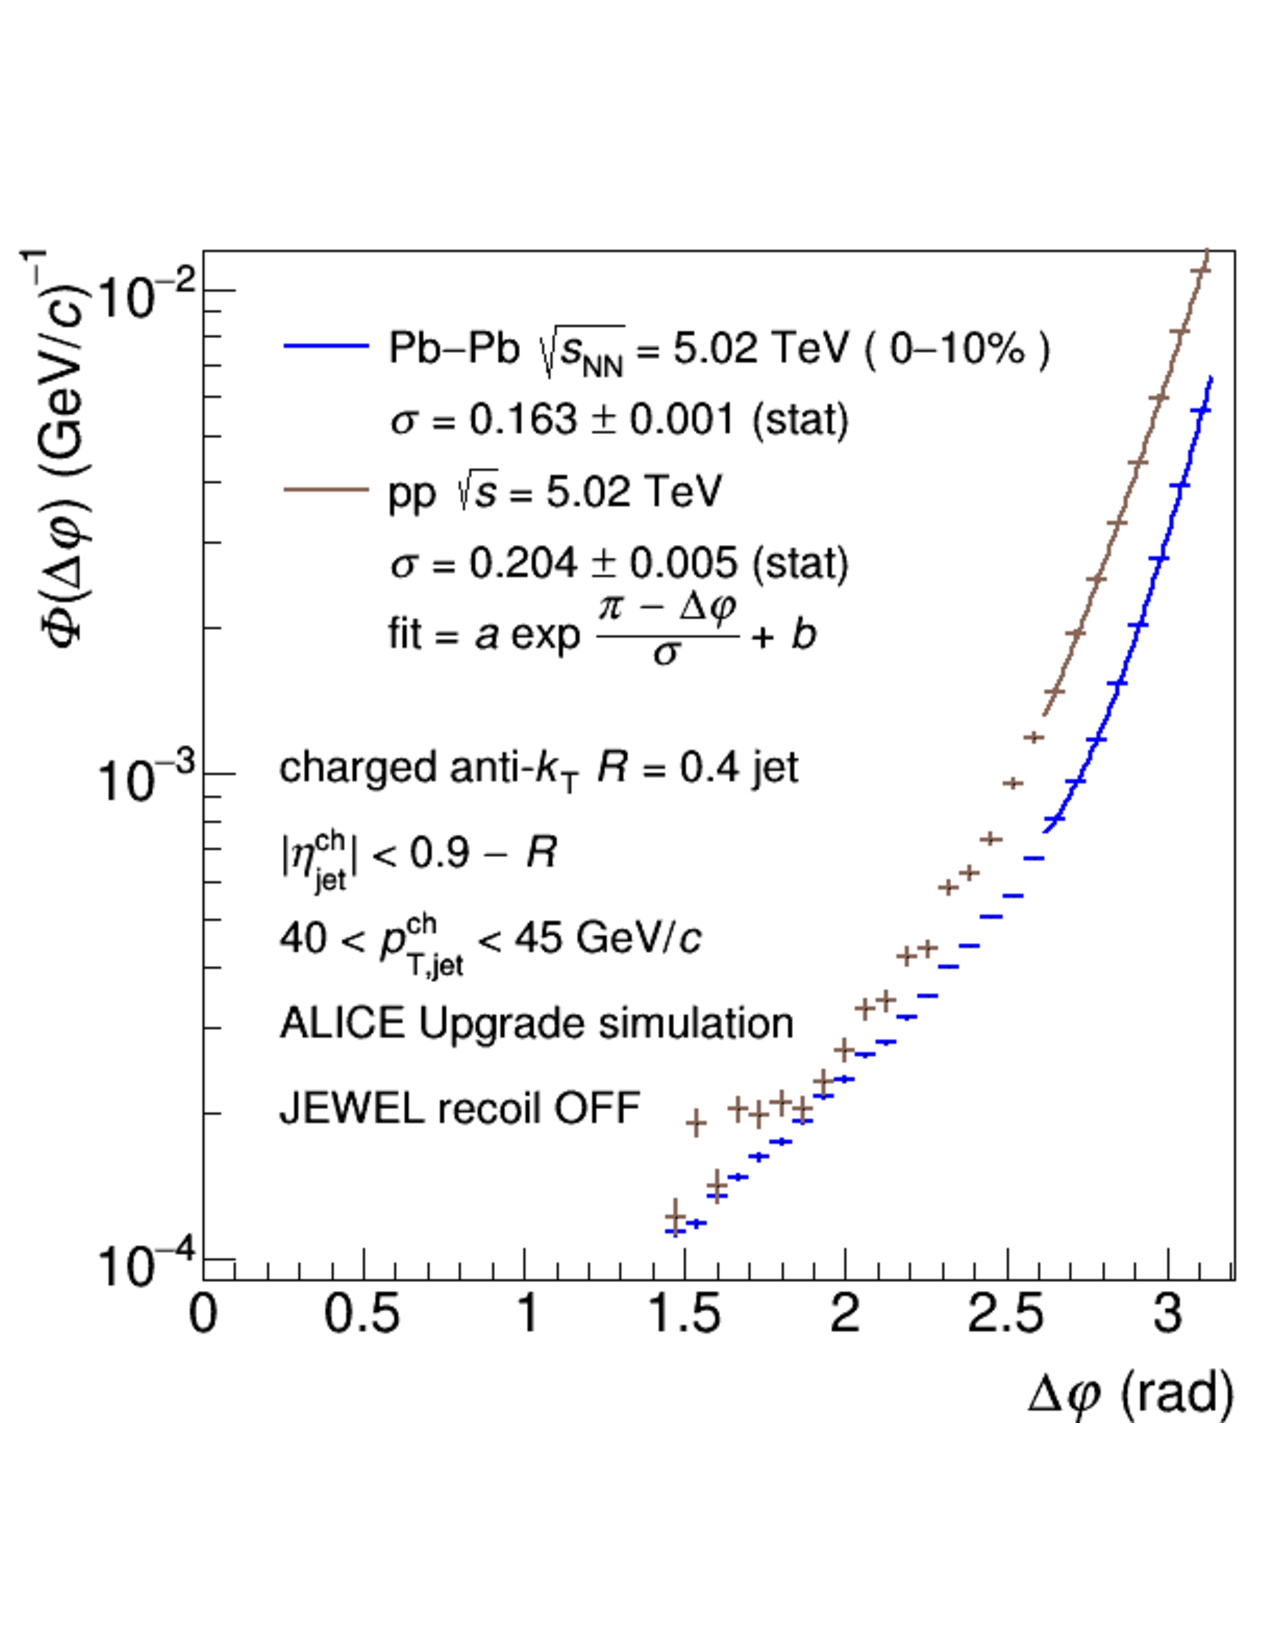
\includegraphics[width=0.6\textwidth]{\main/jets/figures/jetdeflection/JetDeflectionFig_Phi.pdf}
\caption{\jewel\ simulation of the angular distribution of charged jet yield in the ALICE acceptance for  $40<\ptjetch<45$ \gevc\ and $R=0.4$ recoiling from a high-\pt\ reference hadron ($20<\ptt<50$ \gevc), for central Pb--Pb collisions at $\sqrtsnn=5.02$ TeV with 10 nb$^{-1}$ int. luminosity, and pp collisions at $\sqrts=5.02$ TeV with 6 pb$^{-1}$ int. luminosity. The recoil jet azimuthal angle \Dphi\ is defined with respect to the reference axis. The observable shown is $\Phi(\Dphi)$ which incorporates statistical suppression of uncorrelated background.
}
\label{fig:JetDeflectionPhi}
\end{figure}
%----------

Figure~\ref{fig:JetDeflectionPhi} shows the recoil jet azimuthal angle, \Dphi, defined with respect to the reference axis~\cite{Adam:2015doa} as simulated by the \jewel\ event generator. The background-corrected azimuthal distribution of recoil jets recoiling from a high-\pT\ hadron, with the statistics expected by ALICE for central Pb--Pb and pp collisions during the HL-LHC phase is shown. The distribution for central Pb--Pb collisions exhibits an overall yield suppression, corresponding to jet quenching, but also a slight narrowing of the main peak at $\Dphi\sim\pi$ and an enhancement at large deflection angle. The narrowing is characterized by extracting the width of the \Dphi distribution which is $0.204 \pm 0.005$ in the pp simulation and $0.163 \pm 0.001$ for the Pb--Pb simulation with \jewel\. 
In order to quantify the difference at large recoil jet deflection angle between pp and central Pb--Pb collisions, we integrate the $\Phi(\Dphi)$ from $\pi/2$ to a threshold angle \dphithresh~\cite{Adam:2015doa},

\begin{equation}
\Sigma(\dphithresh) = 
\int_{\pi/2}^{\pi-\dphithresh}
\Phi(\Delta\varphi)\mathrm{d}\Delta\varphi.
\label{eq:Sigma}
\end{equation}

\noindent
Figure~\ref{fig:JetDeflectionSigma} shows $\Sigma(\dphithresh)$ for the $\Phi(\Dphi)$ distributions in Fig.~\ref{fig:JetDeflectionPhi}, together with their ratio. In this calculation, the value of $\Sigma$ at $\dphithresh=0$ is around 0.5, which is the yield suppression averaged over the full recoil hemisphere. The ratio grows to $\Sigma\sim1$ at $\dphithresh=1.2$, indicating a factor two enhancement in large-angle yield relative to the hemisphere average. The statistics of the measurement are clearly sufficient to measure the effect predicted by this calculation.
%----------
\begin{figure}[tbh!]
\centering
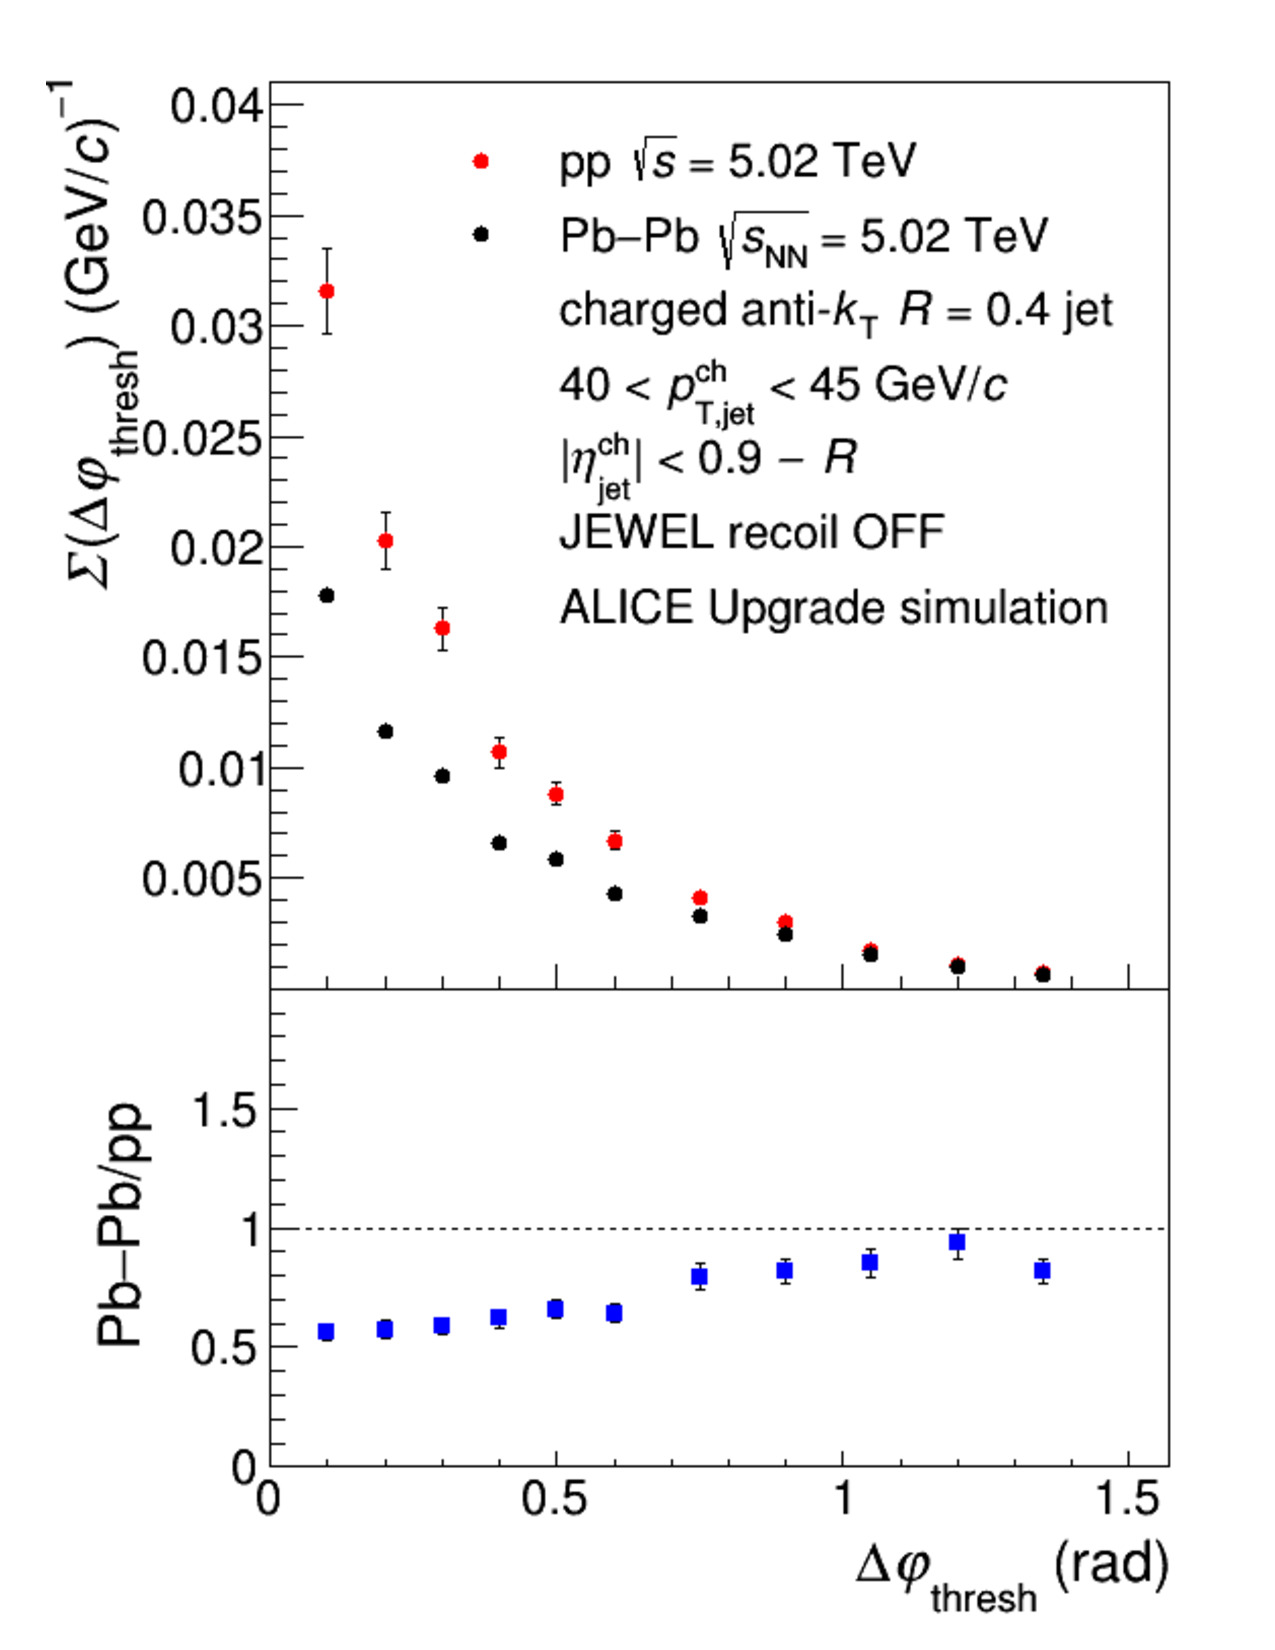
\includegraphics[height=0.6\textwidth]{\main/jets/figures/jetdeflection/JetDeflectionFig_Sigma.pdf}
\caption{Cumulative large-angle yield $\Sigma(\dphithresh)$ (Eq.~\ref{eq:Sigma}) vs. \dphithresh\ for the pp and central Pb--Pb distributions $\Phi(\Dphi)$ in Fig.~\ref{fig:JetDeflectionPhi}. See text for details. 
}
\label{fig:JetDeflectionSigma}
\end{figure}
%----------
However, the calculation in~\cite{Gyulassy:2018qhr} predicts a difference of only a few percent in these distributions for GLV-like and BDMPS-like in-medium scattering, which is more difficult to discriminate. The statistical error in the ratio in Fig.~\ref{fig:JetDeflectionSigma} is around 5\% at $\dphithresh\sim1$, due predominantly to the statistical precision of the pp distribution. %Improvement in the statistical precision of this measurement, needed to achieve a few percent absolute precision, requires larger integrated luminosity for the pp dataset than the value of 6 pb$^{-1}$ used for this calculation. {\it \color{blue} MV: can we say how much? Should we aim for 1\% stat. uncertainty? that would mean 25 times more statistics. This is something that ATLAS and CMS easily can do so we should comment on that. What do you think?\color{black}}{\it \color{red} pmj Nov 5: it would indeed be good for all the experiments to carry out mutually compatible measurements of this type, but that is to be seen. For this report I suggest that we simply truncate the paragraph after "...of the pp distribution." and leave the rest for discussion elsewhere - this section is already too long...Marta, if you agree please make that change...\color{black}}

%As in Sec.~\ref{chapter:smallsystems}, we do not discuss here projections for systematic uncertainties of the jet deflection measurement, since such uncertainties depend crucially on {\it in-situ} detector performance and other factors that are not presently known. We note, however, that the precision of the current jet deflection measurements at low \ptjetch, carried out using the statistical background correction approach, is strongly dominated by statistical error ~\cite{Adam:2015doa,Adamczyk:2017yhe}, and that significant improvement in systematic uncertainties is expected for HL-LHC relative to these initial measurements.  

